\documentclass{article}\usepackage[]{graphicx}\usepackage[]{color}
%% maxwidth is the original width if it is less than linewidth
%% otherwise use linewidth (to make sure the graphics do not exceed the margin)
\makeatletter
\def\maxwidth{ %
  \ifdim\Gin@nat@width>\linewidth
    \linewidth
  \else
    \Gin@nat@width
  \fi
}
\makeatother

\definecolor{fgcolor}{rgb}{0.345, 0.345, 0.345}
\newcommand{\hlnum}[1]{\textcolor[rgb]{0.686,0.059,0.569}{#1}}%
\newcommand{\hlstr}[1]{\textcolor[rgb]{0.192,0.494,0.8}{#1}}%
\newcommand{\hlcom}[1]{\textcolor[rgb]{0.678,0.584,0.686}{\textit{#1}}}%
\newcommand{\hlopt}[1]{\textcolor[rgb]{0,0,0}{#1}}%
\newcommand{\hlstd}[1]{\textcolor[rgb]{0.345,0.345,0.345}{#1}}%
\newcommand{\hlkwa}[1]{\textcolor[rgb]{0.161,0.373,0.58}{\textbf{#1}}}%
\newcommand{\hlkwb}[1]{\textcolor[rgb]{0.69,0.353,0.396}{#1}}%
\newcommand{\hlkwc}[1]{\textcolor[rgb]{0.333,0.667,0.333}{#1}}%
\newcommand{\hlkwd}[1]{\textcolor[rgb]{0.737,0.353,0.396}{\textbf{#1}}}%
\let\hlipl\hlkwb

\usepackage{framed}
\makeatletter
\newenvironment{kframe}{%
 \def\at@end@of@kframe{}%
 \ifinner\ifhmode%
  \def\at@end@of@kframe{\end{minipage}}%
  \begin{minipage}{\columnwidth}%
 \fi\fi%
 \def\FrameCommand##1{\hskip\@totalleftmargin \hskip-\fboxsep
 \colorbox{shadecolor}{##1}\hskip-\fboxsep
     % There is no \\@totalrightmargin, so:
     \hskip-\linewidth \hskip-\@totalleftmargin \hskip\columnwidth}%
 \MakeFramed {\advance\hsize-\width
   \@totalleftmargin\z@ \linewidth\hsize
   \@setminipage}}%
 {\par\unskip\endMakeFramed%
 \at@end@of@kframe}
\makeatother

\definecolor{shadecolor}{rgb}{.97, .97, .97}
\definecolor{messagecolor}{rgb}{0, 0, 0}
\definecolor{warningcolor}{rgb}{1, 0, 1}
\definecolor{errorcolor}{rgb}{1, 0, 0}
\newenvironment{knitrout}{}{} % an empty environment to be redefined in TeX

\usepackage{alltt}
\usepackage{graphicx, color, framed, alltt}
\IfFileExists{upquote.sty}{\usepackage{upquote}}{}
\begin{document}

When performing this analysis on a set of data, we start with the autocorrelation functions of the two channels in each image, and labels of whether these images are bijels or not.

\begin{knitrout}
\definecolor{shadecolor}{rgb}{0.969, 0.969, 0.969}\color{fgcolor}\begin{kframe}
\begin{verbatim}
##      Sample.Number Bijel
## 19              19     n
## 20i            20i     y
## 20ii          20ii     y
## 21              21     n
## 22i            22i     n
## 22ii          22ii     n
\end{verbatim}
\end{kframe}
\end{knitrout}

We then need to turn these functions into a set of single-valued variables that describe features that may separate bijels from non-bijels, such as:

\begin{itemize}
\item The gradient of the particle channel autocorrelation function
\end{itemize}


\begin{knitrout}
\definecolor{shadecolor}{rgb}{0.969, 0.969, 0.969}\color{fgcolor}\begin{kframe}
\begin{alltt}
\hlstd{r} \hlkwb{<-} \hlkwd{c}\hlstd{(}\hlnum{1}\hlopt{:}\hlnum{256}\hlstd{)}
\hlstd{num_points} \hlkwb{<-} \hlkwd{length}\hlstd{(exp_Data}\hlopt{$}\hlstd{Sample.Number)}
\hlstd{y} \hlkwb{<-} \hlstd{exp_Data}\hlopt{$}\hlstd{Autocorrelation.Particle[}\hlnum{1}\hlopt{:}\hlnum{20}\hlstd{]}
\hlstd{lineFits} \hlkwb{<-} \hlkwd{lapply}\hlstd{(}\hlnum{1}\hlopt{:}\hlstd{num_points,}
                  \hlkwa{function}\hlstd{(}\hlkwc{n}\hlstd{)} \hlkwd{lm}\hlstd{(}\hlkwd{unlist}\hlstd{(y[n,])} \hlopt{~} \hlstd{r[}\hlnum{1}\hlopt{:}\hlnum{20}\hlstd{]))}
\hlstd{lineCoeffs} \hlkwb{<-} \hlkwd{lapply}\hlstd{(lineFits,}
                     \hlkwa{function}\hlstd{(}\hlkwc{m}\hlstd{) m}\hlopt{$}\hlstd{coefficients)}
\hlstd{lineGradients} \hlkwb{<-} \hlkwd{lapply} \hlstd{(}\hlnum{1}\hlopt{:}\hlstd{num_points,}
                          \hlkwa{function}\hlstd{(}\hlkwc{p}\hlstd{)} \hlkwd{unname}\hlstd{(lineCoeffs[[p]][}\hlnum{2}\hlstd{]))}
\hlstd{exp_Data}\hlopt{$}\hlstd{Particle.Gradients.20} \hlkwb{<-} \hlkwd{unlist}\hlstd{(lineGradients)}


\hlkwd{library}\hlstd{(ggplot2)}
\hlkwd{ggplot}\hlstd{(exp_Data,}
       \hlkwd{aes}\hlstd{(}\hlkwc{x}\hlstd{=}\hlkwd{as.factor}\hlstd{(Bijel),} \hlkwc{y}\hlstd{=Particle.Gradients.20,} \hlkwc{fill}\hlstd{=Bijel))} \hlopt{+}
       \hlkwd{geom_boxplot}\hlstd{(}\hlkwc{alpha}\hlstd{=}\hlnum{0.3}\hlstd{)} \hlopt{+}
       \hlkwd{geom_jitter}\hlstd{(}\hlkwc{alpha}\hlstd{=}\hlnum{0.5}\hlstd{)} \hlopt{+}
       \hlkwd{xlab}\hlstd{(}\hlstr{"Bijel?"}\hlstd{)} \hlopt{+} \hlkwd{ylab}\hlstd{(}\hlstr{"Gradient"}\hlstd{)} \hlopt{+}
       \hlkwd{ggtitle}\hlstd{(}\hlstr{"Gradient of first 20 points of particle ACF"}\hlstd{)} \hlopt{+}
       \hlkwd{theme}\hlstd{(}\hlkwc{plot.title} \hlstd{=} \hlkwd{element_text}\hlstd{(}\hlkwc{hjust} \hlstd{=} \hlnum{0.5}\hlstd{))}
\end{alltt}
\end{kframe}
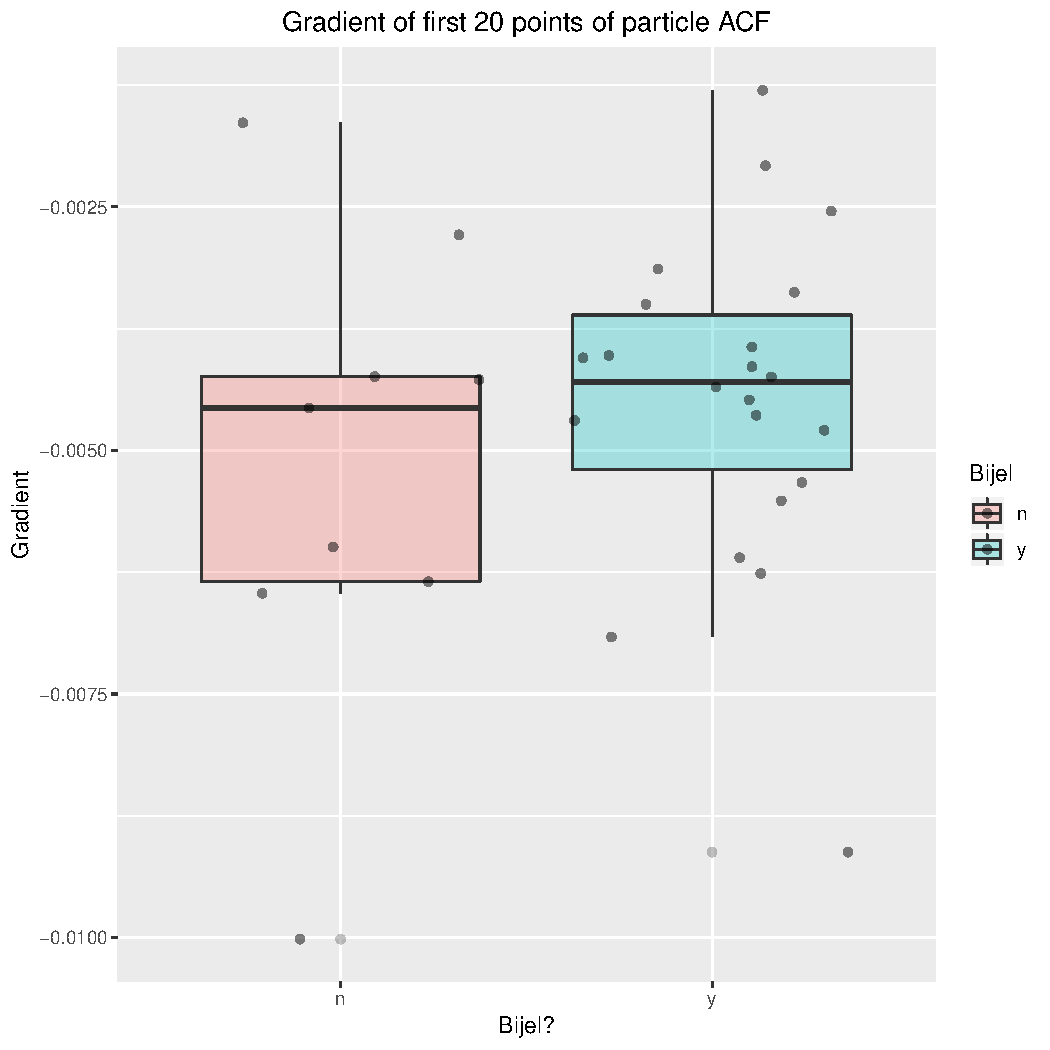
\includegraphics[width=\maxwidth]{figure/unnamed-chunk-2-1} 
\begin{kframe}\begin{alltt}
\hlstd{y2} \hlkwb{<-} \hlstd{exp_Data}\hlopt{$}\hlstd{Autocorrelation.Particle[}\hlnum{1}\hlopt{:}\hlnum{10}\hlstd{]}
\hlstd{lineFits2} \hlkwb{<-} \hlkwd{lapply}\hlstd{(}\hlnum{1}\hlopt{:}\hlstd{num_points,}
                    \hlkwa{function}\hlstd{(}\hlkwc{n}\hlstd{)} \hlkwd{lm}\hlstd{(}\hlkwd{unlist}\hlstd{(y2[n,])} \hlopt{~} \hlstd{r[}\hlnum{1}\hlopt{:}\hlnum{10}\hlstd{]))}
\hlstd{lineCoeffs2} \hlkwb{<-} \hlkwd{lapply}\hlstd{(lineFits2,}
                      \hlkwa{function}\hlstd{(}\hlkwc{m}\hlstd{) m}\hlopt{$}\hlstd{coefficients)}
\hlstd{lineGradients2} \hlkwb{<-} \hlkwd{lapply} \hlstd{(}\hlnum{1}\hlopt{:}\hlstd{num_points,}
                          \hlkwa{function}\hlstd{(}\hlkwc{p}\hlstd{)} \hlkwd{unname}\hlstd{(lineCoeffs2[[p]][}\hlnum{2}\hlstd{]))}
\hlstd{exp_Data}\hlopt{$}\hlstd{Particle.Gradients.10} \hlkwb{<-} \hlkwd{unlist}\hlstd{(lineGradients2)}

\hlkwd{ggplot}\hlstd{(exp_Data,}
       \hlkwd{aes}\hlstd{(}\hlkwc{x}\hlstd{=}\hlkwd{as.factor}\hlstd{(Bijel),} \hlkwc{y}\hlstd{=Particle.Gradients.10,} \hlkwc{fill}\hlstd{=Bijel))} \hlopt{+}
       \hlkwd{geom_boxplot}\hlstd{(}\hlkwc{alpha}\hlstd{=}\hlnum{0.3}\hlstd{)} \hlopt{+}
       \hlkwd{geom_jitter}\hlstd{(}\hlkwc{alpha}\hlstd{=}\hlnum{0.5}\hlstd{)} \hlopt{+}
       \hlkwd{xlab}\hlstd{(}\hlstr{"Bijel?"}\hlstd{)} \hlopt{+} \hlkwd{ylab}\hlstd{(}\hlstr{"Gradient"}\hlstd{)} \hlopt{+}
       \hlkwd{ggtitle}\hlstd{(}\hlstr{"Gradient of first 10 points of particle ACF"}\hlstd{)} \hlopt{+}
       \hlkwd{theme}\hlstd{(}\hlkwc{plot.title} \hlstd{=} \hlkwd{element_text}\hlstd{(}\hlkwc{hjust} \hlstd{=} \hlnum{0.5}\hlstd{))}
\end{alltt}
\end{kframe}
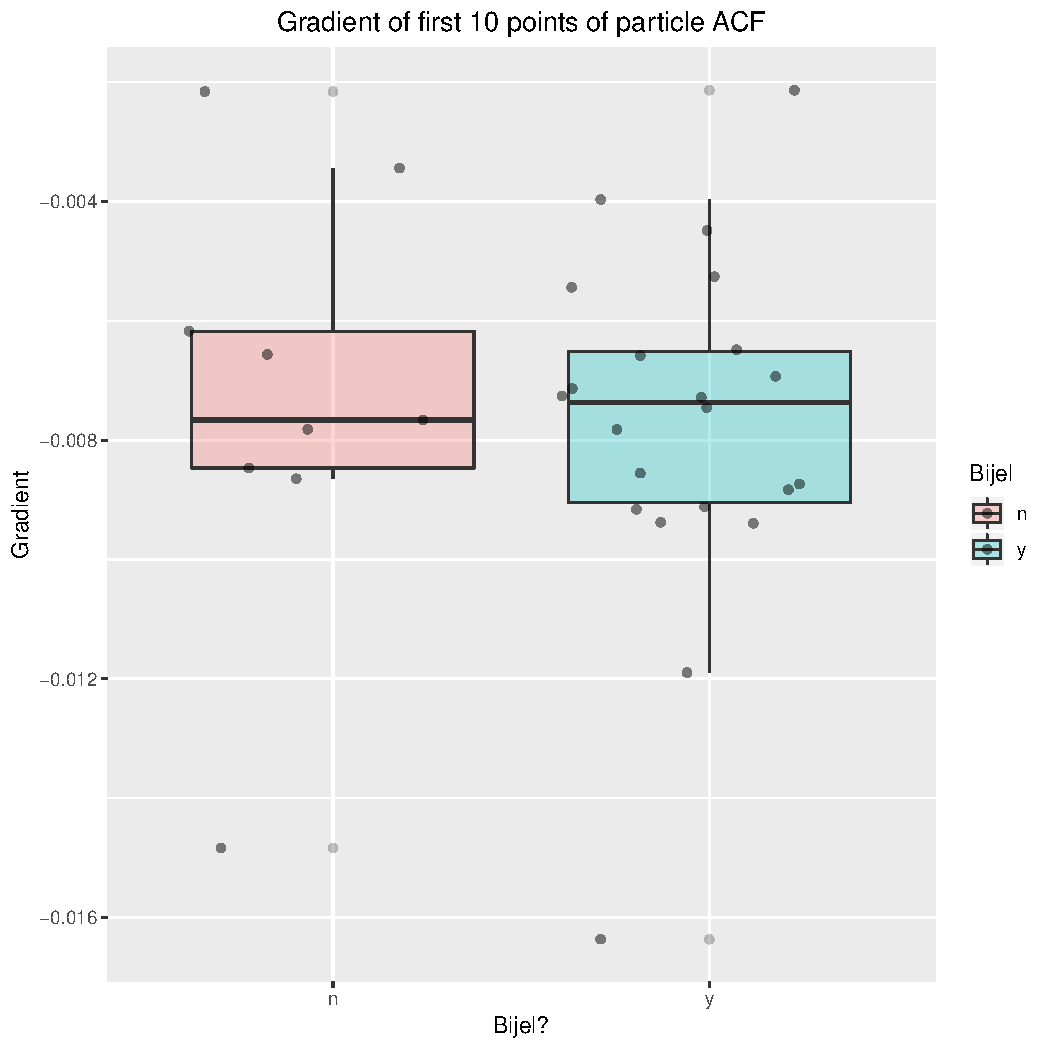
\includegraphics[width=\maxwidth]{figure/unnamed-chunk-2-2} 

\end{knitrout}

\begin{itemize}
\item The position of the first turning point in the liquid channel autocorrelation function
\end{itemize}

\begin{knitrout}
\definecolor{shadecolor}{rgb}{0.969, 0.969, 0.969}\color{fgcolor}\begin{kframe}
\begin{alltt}
\hlkwd{library}\hlstd{(pastecs)}
\hlstd{liquidTurns} \hlkwb{<-} \hlkwd{lapply}\hlstd{(}\hlnum{1}\hlopt{:}\hlstd{num_points,}
                      \hlkwa{function}\hlstd{(}\hlkwc{y}\hlstd{)} \hlkwd{turnpoints}\hlstd{(}\hlkwd{unlist}\hlstd{(exp_Data}\hlopt{$}\hlstd{Autocorrelation.Liquid[y,])))}
\end{alltt}


{\ttfamily\noindent\color{warningcolor}{\#\# Warning in turnpoints(unlist(exp\_Data\$Autocorrelation.Liquid[y, ])): value out of range in 'gammafn'}}\begin{alltt}
\hlstd{firstTurn} \hlkwb{<-} \hlkwd{lapply}\hlstd{(}\hlnum{1}\hlopt{:}\hlstd{num_points,}
                    \hlkwa{function}\hlstd{(}\hlkwc{y}\hlstd{) liquidTurns[[y]]}\hlopt{$}\hlstd{tppos[}\hlnum{1}\hlstd{])}
\hlstd{exp_Data}\hlopt{$}\hlstd{Liquid.First.Turn} \hlkwb{<-} \hlkwd{unlist}\hlstd{(firstTurn)}

\hlkwd{ggplot}\hlstd{(exp_Data,}
       \hlkwd{aes}\hlstd{(}\hlkwc{x}\hlstd{=}\hlkwd{as.factor}\hlstd{(Bijel),} \hlkwc{y}\hlstd{=Liquid.First.Turn,} \hlkwc{fill}\hlstd{=Bijel))} \hlopt{+}
       \hlkwd{geom_boxplot}\hlstd{(}\hlkwc{alpha}\hlstd{=}\hlnum{0.3}\hlstd{)} \hlopt{+}
       \hlkwd{geom_jitter}\hlstd{(}\hlkwc{alpha}\hlstd{=}\hlnum{0.5}\hlstd{)} \hlopt{+}
       \hlkwd{xlab}\hlstd{(}\hlstr{"Bijel?"}\hlstd{)} \hlopt{+} \hlkwd{ylab}\hlstd{(}\hlstr{"Position"}\hlstd{)} \hlopt{+}
       \hlkwd{ggtitle}\hlstd{(}\hlstr{"Position of first turning points of liquid ACF (pixels)"}\hlstd{)}
\end{alltt}
\end{kframe}
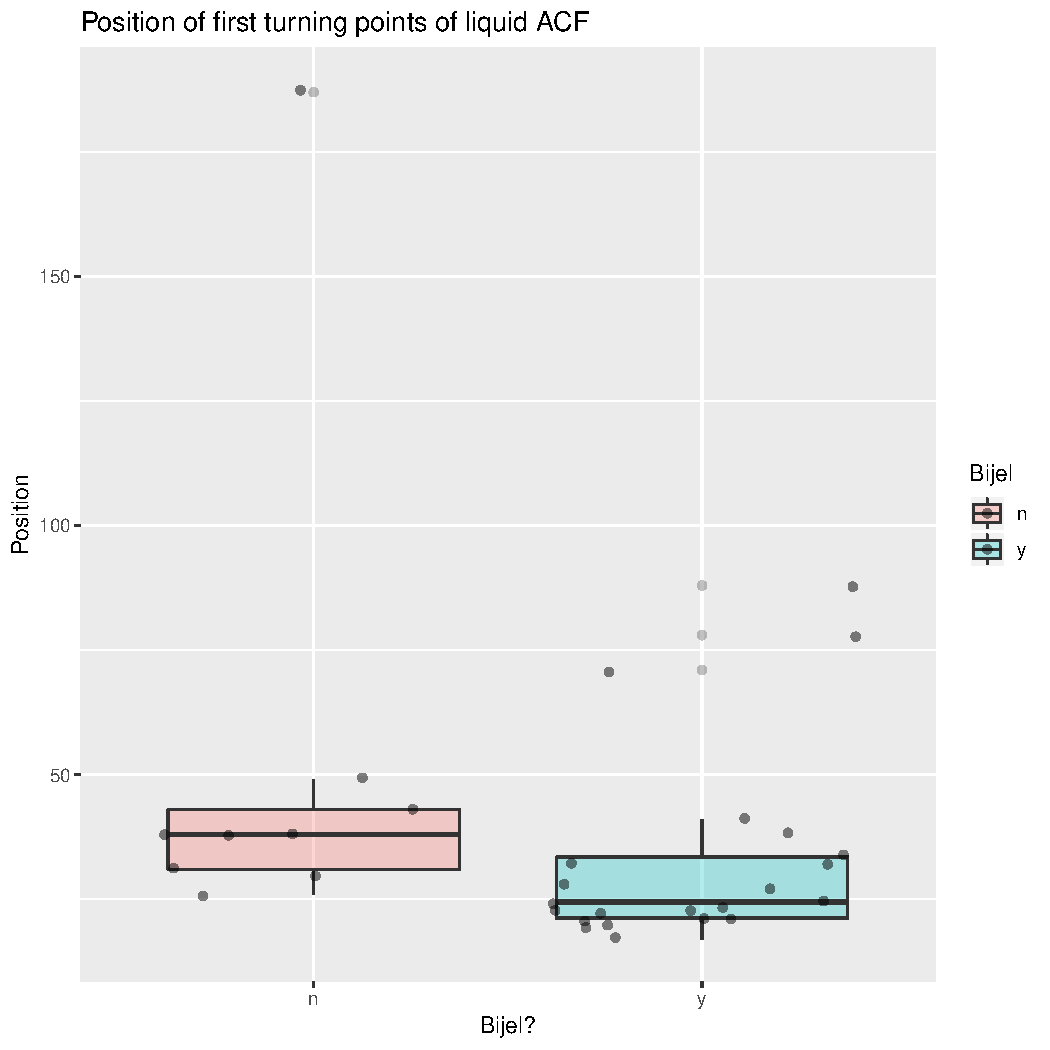
\includegraphics[width=\maxwidth]{figure/unnamed-chunk-3-1} 

\end{knitrout}


\end{document}
